\documentclass[12pt,a4paper]{article}

% Package imports
\usepackage[utf8]{inputenc}        % Allows UTF-8 input
\usepackage{amsmath,amsfonts,amssymb} % For math symbols
\usepackage{graphicx}               % For including graphics
\usepackage{hyperref}               % For hyperlinks
\usepackage{geometry}               % Set page dimensions
\usepackage{fancyhdr}               % For custom headers/footers
\usepackage{enumitem}               % For custom lists
\usepackage{setspace}               % For line spacing
\usepackage{titlesec}               % For section formatting
\usepackage{booktabs}               % For nicer table formatting
\usepackage{array}                  % For advanced table options
\usepackage{adjustbox}              % For adjusting table width
\usepackage{subcaption}             % Add this to your preamble
\usepackage{float}                  % For float options
\usepackage[
backend=biber,
style=ieee,
citestyle=numeric
]{biblatex}                         % For bibliography
\addbibresource{references.bib}     % Add bibliography file

% Set the margins (adjust as needed)
\geometry{
    top=1in,
    bottom=1in,
    left=1in,
    right=1in,
}

% Customizing the header and footer
\pagestyle{fancy}
\fancyhf{}
\fancyfoot[C]{\thepage}             % Centered page number

% Section title formatting
\titleformat{\section}{\large\bfseries}{\thesection}{1em}{}
\titleformat{\subsection}{\normalsize\bfseries}{\thesubsection}{1em}{}

% Set line spacing
\setstretch{1}

% Title and author (can be customized as needed)
\title{Clustering Algorithm on Mice Protein Dataset}
\author{Leihan Chen}
\date{\today}

% Document starts here
\begin{document}

% \maketitle

% Introduction section
\section{Background}
Mice Protein Expression dataset is a multi-class classification/clustering dataset. 
The dataset consists of 77 proteins/protein modifications of expression level that produced detectable signals in the nuclear fraction of cortex \cite{mpe_342}. 
Two types of mice, control (38) and trisomic (34) were used in the experiment. 15 Measurements were taken for each protein across each sample. Therefore, the dataset contains 1080 instances per protein \cite{Higuera2015SelfOrganizingFM}.
The eight classes of mice are then described based on three categorical features genotype, behavior and treatment. In summary, the dataset contains 1080 instances with 77 different protein modifications (features) with 8 types of mice.

The data is obtained from the UCI Machine Learning Repository \cite{mpe_342}. This dataset can be applied as both a multi-class classification and clustering problem. In this report, the dataset is treated as a clustering problem. 
The goal is to cluster the mice samples based on the protein expression levels. This dataset is challenging due to the high dimensionality. 
Meanwhile, the number of instances is relatively small, which is suitable for some clustering algorithms such as Hierarchical Clustering. A visualization of the dataset (features are reduced to 2 for visualization purposes) is shown in the subfigure of figure \ref{fig:comparison_clustering}.

% A visualization of label distribution is shown in figure \ref{fig:label_distribution}. It is clearly observed that the class is imbalanced, with the largest class being with 3546 instances while the smallest only contains 522 instances.
% Moreover, figure \ref{fig:dry_bean_violin} shows the violin plot of each feature (all features are normalized for visualization convenience). 
% The figure demonstrates that the dimensional features are approximately normally distributed while the shape features are opposite. Meanwhile, some features such as Solidity, ConvexArea, and AxisLength have some significant outliers.

% Methodology section
\section{Methods}\label{sec:methods}
\subsection{Pre-processing}\label{subsec:preprocessing}
It is noticed that the dataset has missing values in many features. Therefore, the missing values are imputed with K Nearest Neighbors (KNN) imputer \cite{scikit-learn_KNNImputer}. 
After imputation, a QuantileTransformer \cite{scikit-learn_QuantileTransformer} is applied to the dataset to normalize the features. 
The motivation for using QuantileTransformer is that it can transform the features to follow a uniform or normal distribution, 
which contributes to equal weight for distance-based clustering algorithms, and avoids the effect of some extreme outliers too.

After the quantile transformation with uniform output distribution, the features are reduced with Principal Component Analysis (PCA) \cite{MACKIEWICZ1993303} to reduce the dimensionality. 
This is useful to decorrelate the features and reduce the computational complexity of the clustering algorithms. Here, the PCA algorithm will only keep the first several principal components to retain 75\% of the variance. 
Finally, a robust scaler \cite{scikit-learn_RobustScaler} is applied to the dataset to standardize the features.

\subsection{Clustering Algorithms}\label{subsec:clustering}
Three clustering algorithms are applied to the pre-processed dataset, including KMeans, DBSCAN and Agglomerative Clustering. 
With the setting of KMeans, the number of clusters is set to 8, which is the number  of classes in the dataset. Considering the complexity of the dataset, we initial cluster centroids using sampling based on an empirical probability distribution of the points' contribution to the overall inertia. 
Moreover, fix number of times the k-means algorithm is run with different centroid seeds is set to 10.

For DBSCAN, to determine the optimal hyperparameters, We use the elbow method to find the optimal value of epsilon. Specifically, the K-distance graph is computed to find the elbow point with a proposed method \cite{kneedle_python} in 2011. 
The minimum number of samples is empirically set to 5. Also, we set an additonal eps modifier to adjust epilson values if needed.

Regarding the setting of Agglomerative Clustering, the linkage is set to 'ward' to minimize the variance of the clusters being merged. Also, the number of clusters is set to 8.

\subsection{Evaluation}\label{subsec:evaluation}
The performance of the abovementioned clustering algorithms is evaluated with different metrics \cite{scikit-learn_clustering}. 
With the given ground truth labels,the homogeneous score and completeness score are evaluated to reflect the purity of the given cluster and given class, respectively.
Moreover, the V-measure score is calculated to reflect the harmonic mean of homogeneity and completeness. 
Additionally, the adjusted rand index and adjusted mutual information are computed to reflect the similarity between the true labels and the predicted labels. 
Another common metric, silhouette score, is also utilized to reflect the compactness of the clusters. 
Lastly, Separation (SSB) and coherence (SSE) are specifically targeted for KMeans to evaluate the inter-cluster and intra-cluster sum of squares, respectively.



% Results section
\section{Results}\label{sec:results}
The direct visual comparison of three clustering algorithms with ground truth is shown in figure \ref{fig:comparison_clustering}. 
KMeans and Agglomerative Clustering achieve similar performance, while the result of DBSCAN has two significant dominant clusters. 
The clustering result of DBSCAN is under-clustered for two clusters, and over-clustered for the rest of the clusters.

The visualization of three clustering algorithms can be found in figure \ref{fig:clustering_visualization}. 
The subfigure \ref{fig:kmeans_visualization} shows the clustering result of KMeans, applied on a two-dimensional PCA-reduced dataset. It is observed that KMeans can separate the clusters relatively well.
The dendrogram of Agglomerative Clustering is shown in subfigure \ref{fig:dendrogram_distribution}. 
The dendrogram clearly illustrates that some subclusters on the left side of the dendrogram with orange connecting lines are merged into one cluster. 
This also explains the relatively low performance in its homogeneity score.

The metrics of three clustering algorithms are represented in table \ref{tab:clustering_results}. 
All of three algorithms cannot achieve an impressive performance, with the relatively best performance of Agglomerative Clustering, only achieves 0.32 in V-Measure. 
Considering the complexity of the dataset observed in figure \ref{fig:comparison_clustering}, both distance-based clustering algorithms, DBSCAN and Agglomerative Clustering, or density-based clustering algorithm, DBSCAN, fail to separate the clusters accurately. 
It is also noticeabe that DBSCAN performance is higher on all metrics except for the silhouette score, which is negative. 
The reason behind it is that DBSCAN over clusters the dataset and there is a number of noise points too. All of them contributes to the decrease of silhouette score. 
Also, the algorithm is very sensitive to the hyperparameters, and the elbow method is not always applicable to finding the optimal hyperparameters.

\section{Conclusion}\label{sec:conclusion}
To conclude, three different clustering algorithms are applied to challenging Mice Protein Expression dataset. 
The KMeans and Agglomerative Clustering algorithms achieve similar performance, while DBSCAN has the issue of both under and over clustering on certain classes. 


% References section
\printbibliography


% Appendix section for all tables and figures
\section{Appendix}\label{sec:appendix}
% Compare the clustering results of three algorithms
\begin{figure}[H]
    \centering
    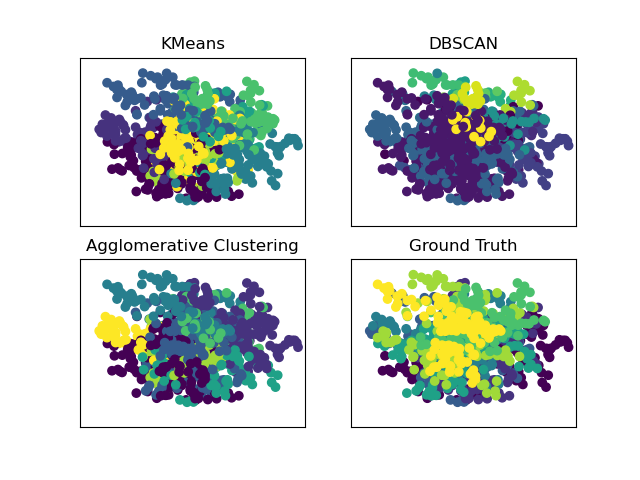
\includegraphics[width=0.9\textwidth]{figures/clustering_result_comparison.png}
    \caption{The comparison of clustering algorithms (features are reduced to two dimensions)}
    \label{fig:comparison_clustering}
\end{figure}

% Get three subfigures vertically aligned
\begin{figure}[H]
    \centering
    \begin{subfigure}[b]{0.3\textwidth}
        \centering
        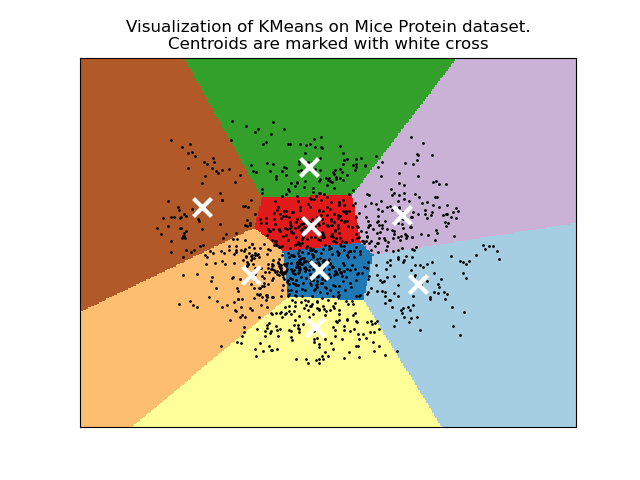
\includegraphics[width=\linewidth, height=4cm]{figures/kmeans_vis.png}
        \caption{KMeans clustering}
        \label{fig:kmeans_visualization}
    \end{subfigure}
    \hfill
    \begin{subfigure}[b]{0.3\textwidth}
        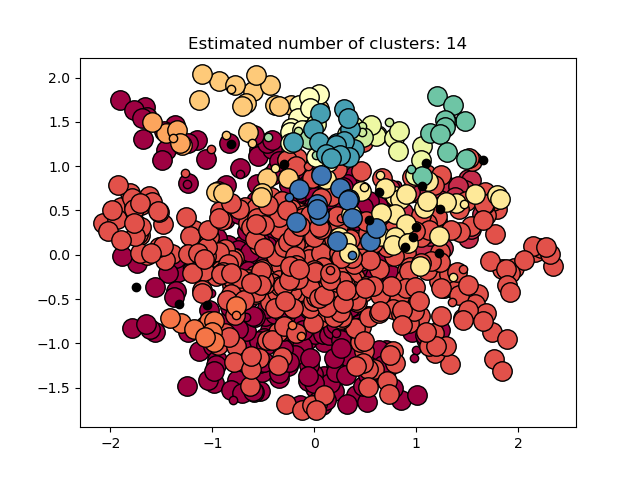
\includegraphics[width=\linewidth, height=4cm]{figures/dbscan_vis.png}
        \caption{DBScan clustering}
        \label{fig:dbscan_visualization}
    \end{subfigure}
    \hfill
    \begin{subfigure}[b]{0.3\textwidth}
        % set two figures height identical
        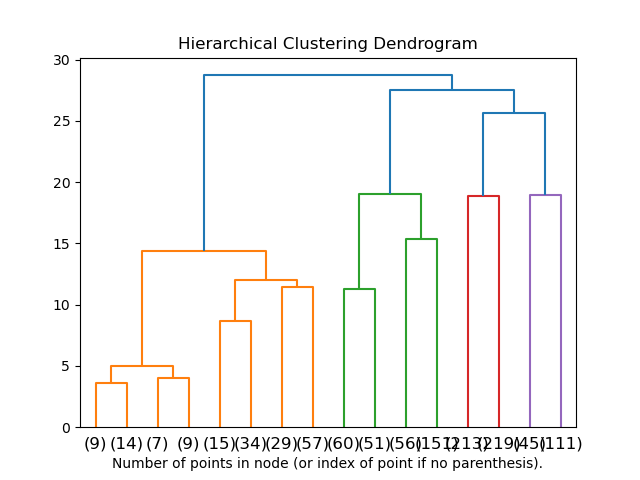
\includegraphics[width=\linewidth, height=4cm]{figures/dendrogram_vis.png}
        \caption{Dendrogram of Agglomerative Clustering}
        \label{fig:dendrogram_distribution}
    \end{subfigure}
    \caption{Visualization of three clustering algorithms}
    \label{fig:clustering_visualization}
\end{figure}

% \vspace{-1em} % Adjust the value as needed to reduce the space

% A table to show the clustering results on different metrics, make the table within one page width
\begin{table}[H]
\begin{adjustbox}{width=\textwidth}
    \centering
    \begin{tabular}{lccccccccc}
        \toprule
        \textbf{Algorithm} & \textbf{Time} & \textbf{Separation} & \textbf{Cohesion} & \textbf{Homogeneity} & \textbf{Completeness} & \textbf{V-measure} & \textbf{ARI} & \textbf{AMI} & \textbf{Silhouette Score} \\
        \midrule
        KMeans & 0.372s & 2048.635 & 1945.001 & 0.291 & 0.296 & 0.294 & 0.150 & 0.286 & 0.193 \\
        DBSCAN & 0.024s & \textbackslash & \textbackslash & 0.439 & 0.543 & 0.486 & 0.230 & 0.469 & -0.018 \\
        Agglomerative Clustering & 0.009s & \textbackslash & \textbackslash & 0.311 & 0.329 & 0.320 & 0.151 & 0.312 & 0.126 \\
        \bottomrule
    \end{tabular}
\end{adjustbox}
    \caption{Clustering results on different metrics}
    \label{tab:clustering_results}
\end{table}

\end{document}